\section{软件测试}

    根据本次毕业设计中的实现内容,软件测试主要分为两大部分,系统功能模块测试及系统整体测试,其中功能模块测试主要包含
    指纹识别模块测试,网卡驱动测试,网络协议栈集成测试几个部分。

    \subsection{指纹识别模块测试}

    本测试主要在上位机中进行,主要目的在于证明可以通过指纹管理程序在不影响指纹识别的情况下
    对于指纹特征数据进行上传和下载(见图\ref{总体设计图})右侧上位机与 FPM383C 之间的连线。

    \subsubsection*{测试准备:}
    硬件层面上需要使用 CH340 TTL转USB模块,杜邦线,指纹识别模块,开发板。
    软件层面上不需要额外准备,直接采用 chainboot 显示对应输出即可。

    经串口发送亮灯信号,对应指纹模块亮灯可见指纹识别模块能与计算机和树莓派建立有效的串口连接。

    \subsubsection{指纹注册测试}
    
    由于按照目前设计,指纹注册功能在上位机中实现。在正确注册指纹之后,通过调用协议使指纹模块上传
    指纹特征信息到上位机,通过 UdpSocket 将对应数据包中信息整合后经过网络分发到下位机
    \footnote{在这段测试中,由于经由网络下发指纹特征信息由于量太多不太容易进行呈现,暂且不进行相关演示}。

    首先通过指纹识别模块配的客户端程序清空上位机从属指纹模块中的指纹模板(如图\ref{fig::清空指纹模板})。

    \begin{figure}[ht]
        \centering
        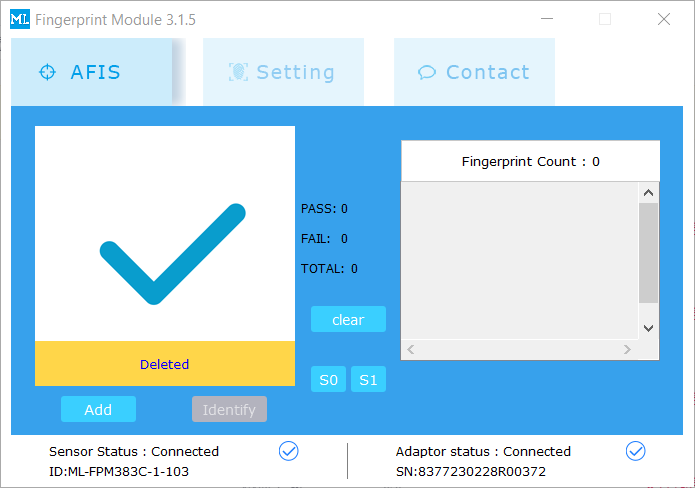
\includegraphics[scale=0.8]{./imgs/清空指纹模板.png}
        \caption{清空指纹模板}    \label{fig::清空指纹模板}
    \end{figure}

    将指纹模块插入到上位机中,通过在上位机中运行的简单注册终端进行注册。
    首先,根据用户信息表(见表\ref{tab:userInfo})中所设计的各项信息进行输入,在输入数据完成校验。
    然后,管理程序调用指纹注册函数,函数在调用指纹模块的自动注册命令完成有关指纹模块的注册后
    自动调用上传指令,
    将对应数据由上位机从属指纹识别模块上传到上位机数据库中 Finger{id}Data 表中
    (见图\ref{test::用户注册} \footnote{图中下半部分输出的字节数据分别代表由串口获取的完整特征信息和其中的指纹信息}),
    并且根据数据库设计,自动完成 users,FingerInfo 等关联表的构建。

    \begin{figure}[ht]
        \centering
        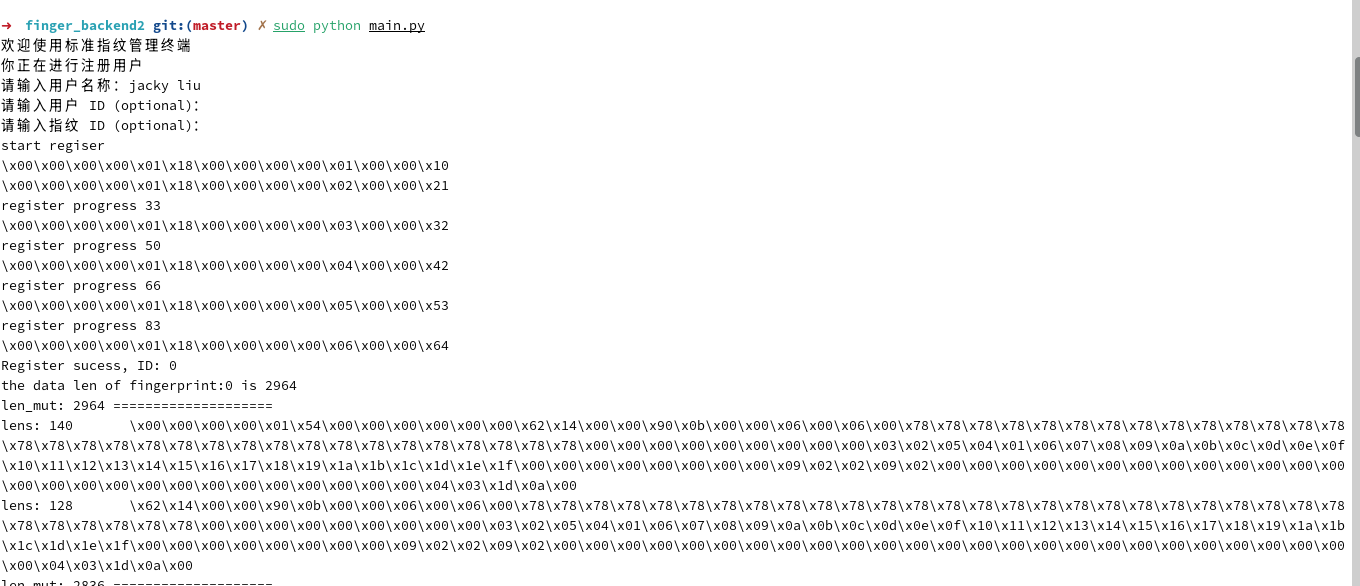
\includegraphics[width=\textwidth]{./imgs/测试-用户注册.png}
        \caption{用户注册}    \label{test::用户注册} 
    \end{figure}   

    完成注册操作之后,由图\ref{test::注册后数据库查询} 可见,对应的表和关系已经正确构建。
    下图中对 FingerInfo 表的查询体现了 finger\_id 0 与 user\_id 1 的映射关系,还保存了指纹特征 0 的长度信息,
    注册的指纹特征信息二进制数据被保存在 Finger0Data 表中。

    \begin{figure}[ht]
        \centering
        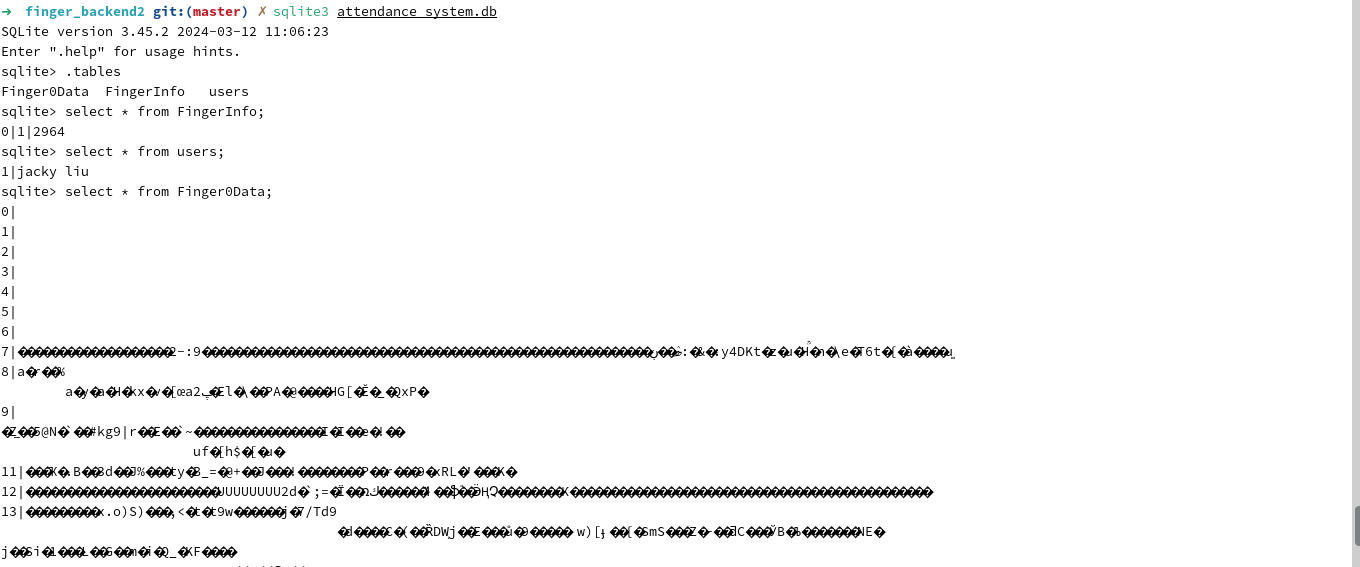
\includegraphics[width=\textwidth]{./imgs/测试-注册后数据库查询.png}
        \caption{用户注册后数据库查询}    \label{test::注册后数据库查询}
    \end{figure}   

    \subsubsection{指纹删除}

    指纹删除功能终端尚未实现,还需要一些时间。

    \subsubsection{指纹下载}

    本测试不属于指纹考勤管理系统的主要组成成分,主要目的在于测试在指纹特征数据的上传和下载中是否出现了信息丢失
    导致指纹无法正常识别的现象。

    首先,先根据指纹注册测试的方式或者是由指纹模块配的指纹管理程序完成指纹注册(见图\ref{fig::注册指纹})后单独进行指纹上传操作。
    然后,由指纹模块配的指纹管理程序删除注册的指纹(见图\ref{fig::清空指纹模板})
    \footnote{删除测试的方法会一并删除指纹特征文件与关联图等内容}。

    \begin{figure}[ht]
        \centering
        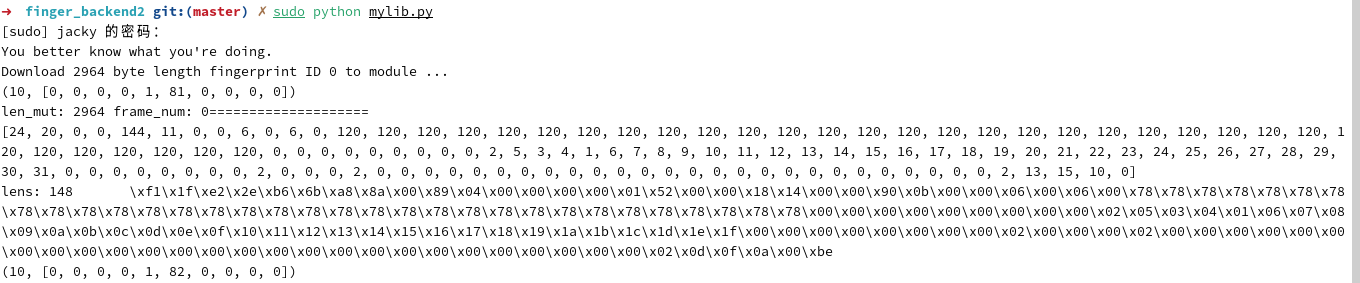
\includegraphics[width=\textwidth]{./imgs/测试-指纹上传.png}
        \caption{指纹上传}    \label{test::指纹上传}
    \end{figure}   

    \noindent
    \begin{minipage}[t]{0.48\linewidth}
        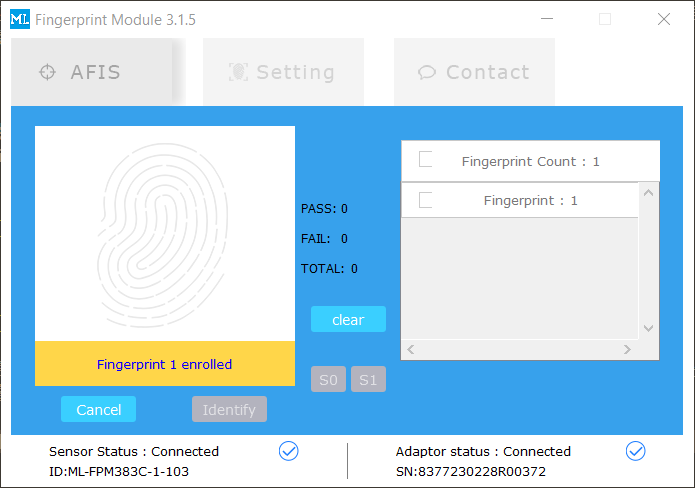
\includegraphics[width=\textwidth]{./imgs/注册指纹.png}
        \captionof{figure}{指纹客户端注册指纹}    \label{fig::注册指纹}
    \end{minipage}
    % \quad
    \begin{minipage}[t]{0.48\linewidth}
        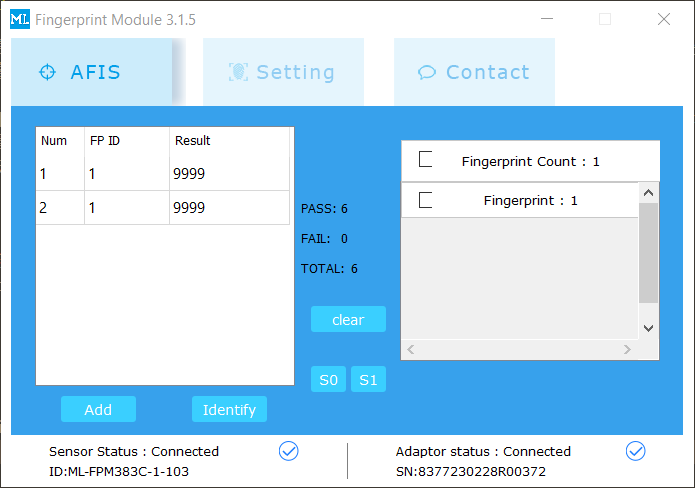
\includegraphics[width=\textwidth]{./imgs/测试-指纹上传后查询与匹配.png}
        \captionof{figure}{指纹上传后查询与匹配}    \label{test::指纹上传后查询与匹配}
    \end{minipage}

    如图 \ref{test::指纹上传} 可见通过执行内置指纹上传函数实现的指纹上传输出,
    其中 (10, [ ..., 0, 81, ... ]) 代表执行 upload 指令时的回返信息,
    第一段数组代表由数据库中读取的二进制指纹特征信息(一帧),
    第二段字节代表整个由上位机经由串口下发到指纹识别模块的串口信息。

    将指纹识别模块重新接入上位机中(如图\ref{test::指纹上传后查询与匹配})可见,
    之前删除的左手大拇指指纹已经重新被识别出来了,并且经过两次指纹匹配测试均能保证
    识别准确率能够达到 100,这无疑证明了在指纹特征信息由指纹模块中上传再下载的过程中
    并没有对于指纹特征信息的完整性进行破坏,上传再下载的行为也不会导致指纹特征信息被破坏。

    \subsection{以太网卡驱动测试}

    在本章节中主要完成了对于网卡驱动的测试工作,其中首先在两台 PC 电脑之间运行 C 语言的收发包脚本,对于脚本
    的功能以及效果进行测试,然后在树莓派原生 Linux 下运行发包脚本,PC 电脑上运行收报脚本以对于树莓派的传输速率进行分析,
    最后,在 ArceOS 上直接发送以太网帧到 PC 机上的接受脚本中测试 ArceOS 网卡驱动的收发包效果。

    \subsubsection{测试脚本测试}

    按照测试计划,采用两台电脑先对测试脚本本身能否完整实现功能进行测试,一台电脑通过 WSL(windows subsystem of linux) 
    运行 linux 测试发包脚本,另外一台笔记本通过 RJ45转USB模块\footnote{或者说叫做usb网卡}
    经由双绞线与前者进行连接,接受对应数据包。

    但是进行测试的时候,实际上并没有办法实现以太网帧的收发,
    经过分析之后发现产生这种问题的主要原因的是 WSL 与 宿主机 之间的网络连接方式是通过
    类似于 NAT(Network address translation) 的方式进行连接的,在这种情况下,WSL 与 宿主机之间存在一个子网,因此
    在 WSL 中在以太网帧层面实现的收发只能在,并不能在宿主机上获得转发,因此
    另外一台 linux PC 没有办法收到对应以太网帧
    \footnote{IP层以上的包会自动被转发,但以太网帧不会}。

    最终,采用了两台运行 linux 操作系统的电脑进行此测试(其中一台采用 nixos live,一台是 nixos)其连接如下图 \ref{tests::测试脚本测试连接图}所见。
    \footnote{由于其中一台仍通过 RJ45转USB模块 实现网络收发功能同时配有百兆网卡,因此本次测试中的最高传输速率仅为100mbps}
    二者均在完全关闭防火墙,配置对应以太网卡的 ip 地址,并实现相互 ping 之后展开测试。
    发包侧(如附录代码段 \ref{code::eth-send})在十秒内持续发送以太网帧,并且在以太网帧的第 16 位开始的八个字节添加代表当前以太网帧序号的八个字节 (unsigned long long)数据。
    收包侧(如附录代码段 \ref{code::eth-recv})按照对应收包顺序与检测出的序号综合进行判断在传输过程中是否存在丢包,乱序的情况。

    \begin{figure}[ht]
        \centering
        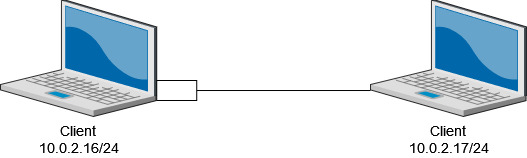
\includegraphics[scale=0.6]{imgs/测试脚本测试连接图.jpg}
        \caption{测试脚本测试连接图}    \label{tests::测试脚本测试连接图}
    \end{figure}

    具体测试结果见下 4-1 \ref{test::测试脚本测试}表,在以太网帧百兆层面不存在丢包的情况,可以较好的实现收发包测试效果。

    \begin{table}[ht]
    \centering
    \label{tests::测试脚本测试}
    \caption{测试脚本测试表}
    \csvautobooktabular{./imgs/测试记录-测试脚本测试.csv}
    \end{table}

    \subsubsection{树莓派网络传输速率测试}

    本测试主要想要实现的效果在于测试出在树莓派直接采用 Linux 镜像原装的网卡驱动所能实现的传输效率,以方便与后面
    我们通过 Rust 在 ArceOS 裸机上实现的网卡驱动(以太网帧)测试出的收发效率进行对比。

    在具体测试操作上,除了其中一台百兆网卡的测试PC被更换成为了树莓派外基本与前章节(测试脚本测试)保持一致。
    
    \begin{figure}[ht]
        \centering
        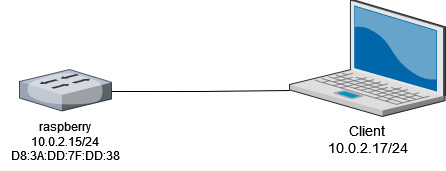
\includegraphics[scale=0.6]{imgs/树莓派-测试机连接.jpg}
        \caption{树莓派-测试机连接图}    \label{tests::树莓派测试机连接图}
    \end{figure}


    此处采用以太网帧作为其中一个测试参数主要是考量到在测试的过程中采用死循环不断发送的方法,
    单个以太网帧长度越长,在发送该以太网帧花费的传输时间就越长
    \footnote{由于拷贝,寄存器操作等导致},
    花费在帧与帧之间切换的时间就越短,更能测试出以太网驱动的极限网络吞吐量。

    在进行测试的时候采用如下算法对于以太网传输速率进行评估,其中 total\_bytes 代表在测试时间内完成传输的总字节数,elapsed\_secs 代表总测试时间。
    经过测试,(测试记录见附录表 \ref{tests::Linux驱动传输速率测试}),将每组数据取平均值之后可做出如下图像(如图 \ref{tests::Linux网卡驱动传输率与以太网帧大小} 所示)

    由图可知,前文提出的以太网帧与网络传输速率之间的关系基本正确,二者存在指数关系,且以太网帧越大,在同等时间内的以太网传输速率越大。
    在以太网帧层面网络传输速率最大能达到 983.21 MBps\footnote{以太网帧总长度 1500 字节情况下},接近树莓派千兆网卡的理论最大传输速率 1000 MBps。

    $$\text{mbps} = \frac{\text{total\_bytes} \times 8.0}{\text{elapsed\_secs} \times 1,000,000.0}$$

    \begin{figure}[ht]
    \begin{tikzpicture}
        \centering
        \begin{axis}[
            xlabel={以太网帧大小}, ylabel={传输速率},
            xmin=0,
            width=0.8\textwidth,
            legend pos=south east,
            grid=both
        ]
        
        \addplot[thick, mark=*, blue] coordinates {
            (64, 112.3833333)
            (128, 233.0333333)
            (256, 456.5257143)
            (512, 739.01)
            (1024, 898.616)
            (1280, 943.565)
            (1408, 949.85)
            (1500, 946.8366667)
        };
        \addlegendentry{发送端速率}
        
        \addplot[thick, mark=*, red] coordinates {
            (64, 112.3833333)
            (128, 233.0333333)
            (256, 445.5085714)
            (512, 734.5766667)
            (1024, 889.338)
            (1280, 938.1825)
            (1408, 949.85)
            (1500, 938.5266667)
        };
        \addlegendentry{接受端速率}

        \end{axis}
    \end{tikzpicture}
    \caption{树莓派Linux驱动传输率与以太网帧大小关系图}    \label{tests::Linux网卡驱动传输率与以太网帧大小}
    \end{figure}

    % TODO: 在前期测试中是可以正常发现对应丢包情况的发生的,但是不知道为什么后面无法重现这个问题,暂且删除这个部分的说明

    % 在树莓派进行测试的过程中,根据序号与收包端收报次序的对比,C 接收端程序提示在本次测试中出现了丢包的情况。
    % 经过 Wireshark 对比之后证实确实存在丢包情况。

    % TODO: 在拷贝图片的时候两张图片是一致的li
    % \begin{figure}[ht]
    %     \centering
    %     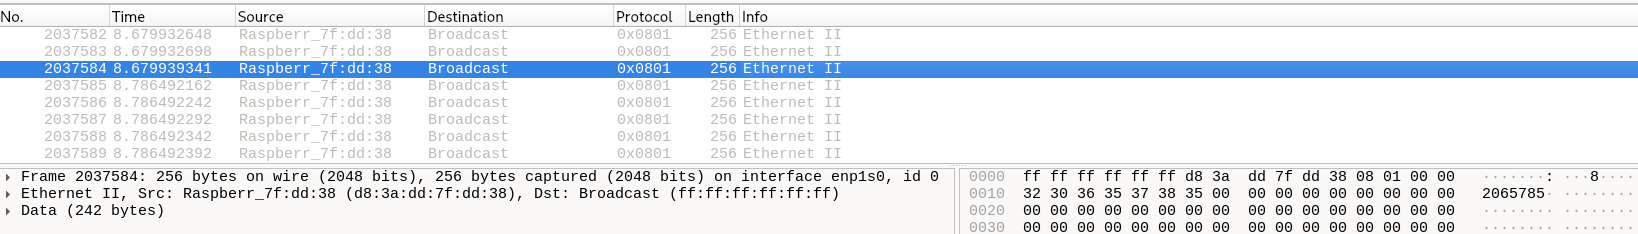
\includegraphics[width=\textwidth]{./imgs/丢包2.png}
    %     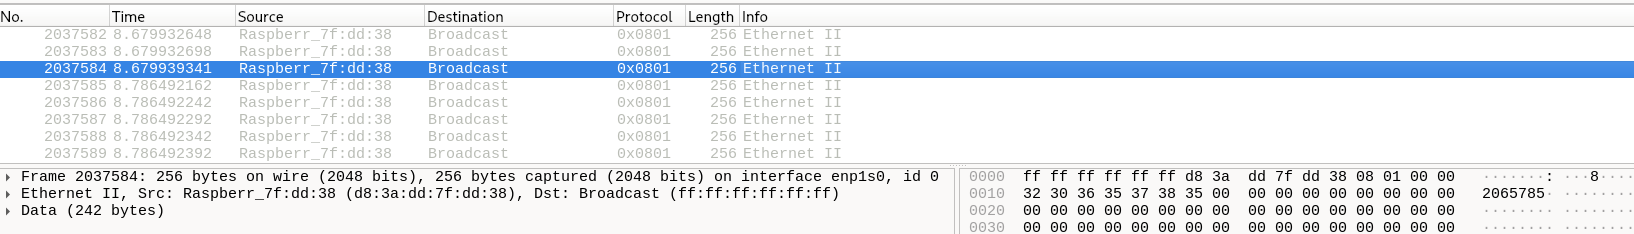
\includegraphics[width=\textwidth]{./imgs/丢包1.png}
    %     \caption{以太网帧发包测试}    \label{test::以太网帧发送}
    % \end{figure}   

    \subsection{网卡驱动测试}

    本测试主要目的在于测试在 ArceOS 下的以太网卡驱动传输速率,并且最终与树莓派网络传输速率进行对比,评价以太网网卡驱动的实现效果。
    由于后面在将以太网卡驱动与 ArceOS 网络协议栈进行嵌合的时候对于以太网卡驱动进行了破坏性修改
    \footnote{BCM54213PE驱动中调用ArceOS函数是通过PhantomData间接调用traits实现来完成的}。
    因此,本次测试由完成了网络驱动测试的 \href{https://bitbucket.org/jackyliu16/arceos/commits/92e9b6abcdf180359381088552688c0fcbc83bf2}{commit} 
    分叉出 \href{https://bitbucket.org/jackyliu16/arceos/commits/branch/ethernet-test}{ethernet-test}
    分支,并在此分支中完成了对应测试。

    \subsubsection{发包测试}

    由树莓派向上位机直接发送以太网帧,在上位机中通过 wireshark 进行抓包(如图\ref{test::以太网帧发送})

    \begin{figure}[ht]
        \centering
        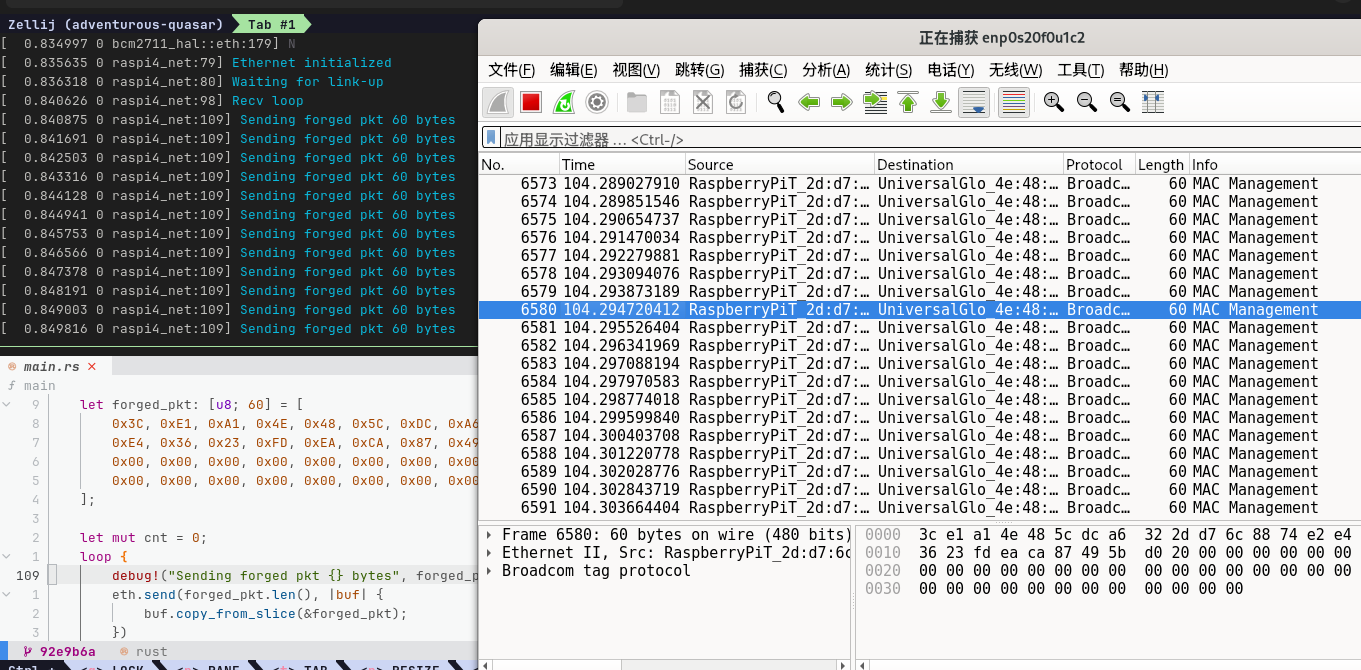
\includegraphics[width=\textwidth]{./imgs/以太网帧通信正常.jpg}
        \caption{以太网帧发包测试}    \label{test::以太网帧发送}
    \end{figure}   

    \subsubsection{收包测试}

    在树莓派上直接收包并打印对应信息(见图\ref{test::以太网帧接收})。
    由于目前树莓派并没有实现网络协议栈,因此
    无法通过如 nc, nping 等基于网络的传输工具向树莓派发送自定义以太网帧。
    因此,此处直接使用了 nc 随便发送了一段数据到树莓派中。
    此处指定的网段与上,下位机网段一致,因此上位机会在同一子网中释放 ARP 探寻包,
    如图 \ref{test::以太网帧接收} 所示,对应的 ARP 探寻包被正确解析,因此可以浅薄的认为以太网驱动可以正常的收到上位机传输的探寻包。
    % TODO: 这个地方其实可以补测试,用前面测试脚本测试的 send_ethernet.c 来发

    \begin{figure}[ht]
        \centering
        \begin{subfigure}
            \centering
            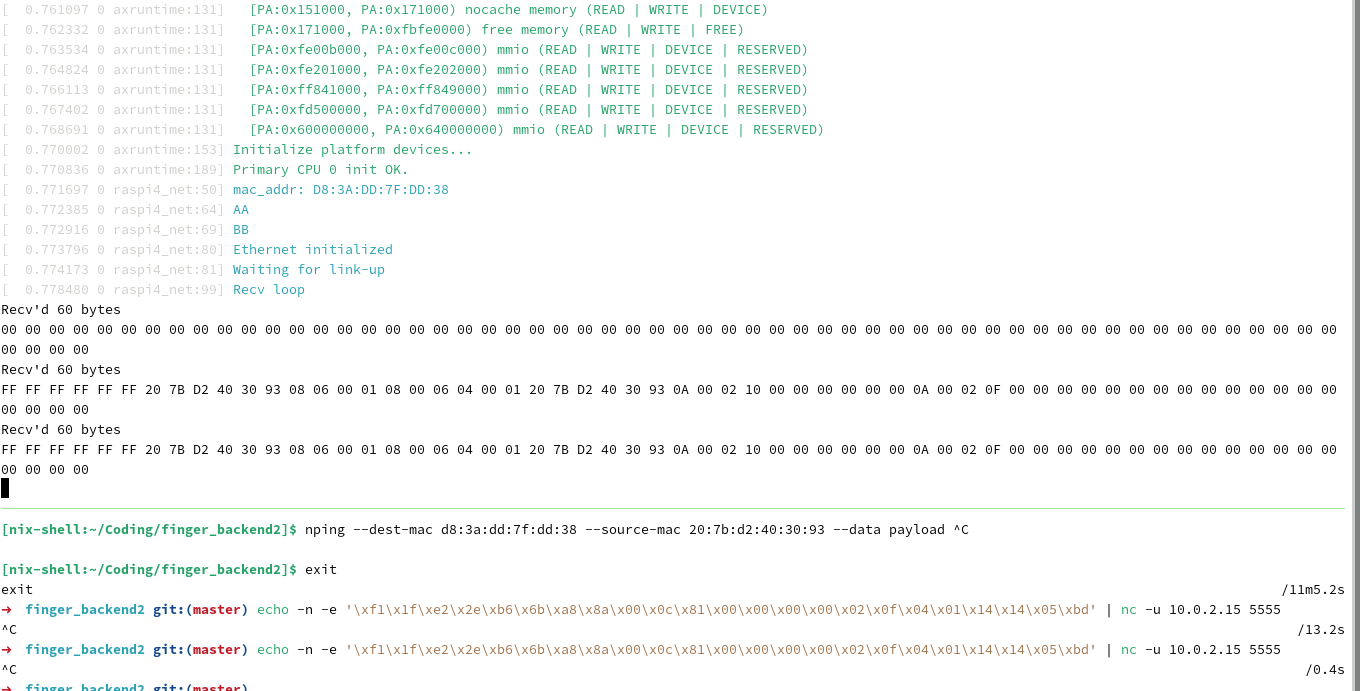
\includegraphics[width=\textwidth]{./imgs/测试-以太网帧接收.png}
        \end{subfigure}
        \hfill
        \begin{subfigure}
            \centering
            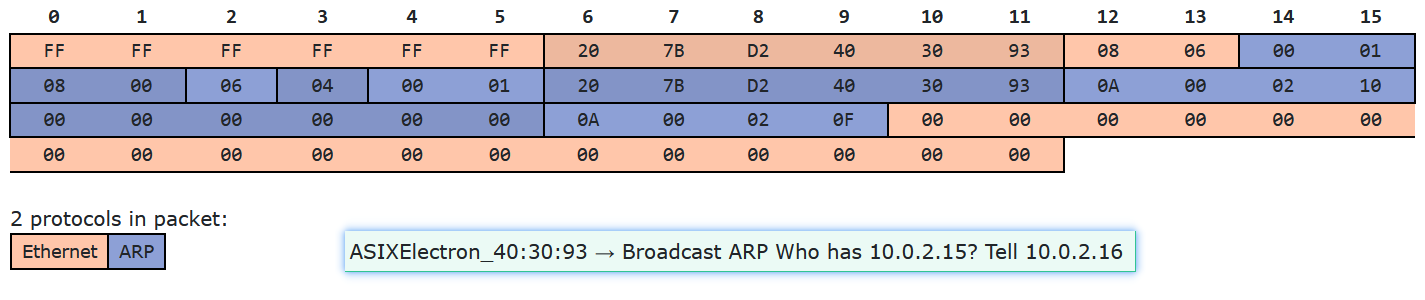
\includegraphics[width=\textwidth]{./imgs/测试-以太网帧接收-解析.png}
        \end{subfigure}
        \caption{接受的以太网帧及解析} \label{test::以太网帧接收}
    \end{figure}

    \subsubsection{传输速率测试}

    前面的测试说明当前以太网帧的收发功能是正常的,此处使用一个简单的发送 buf 的循环尝试对于以太网驱动的传输速率进行测试,
    其实现上类似于前文进行 Linux 原生网卡驱动测试时的操作,直接在以太网帧 16-24 位中插入代表当前序号的纯数字
    \footnote{由于测试脚本测试实现的部分为了方便进行调试,找到中断包,因此直接采用将代表序号的数字经由 snprintf 转换成 char 直接写入到以太网帧中
    ,此处为了保证一致此处采用了同样的方法}。

    $$\text{mbps} = \frac{\text{total\_bytes} \times 8.0}{\text{elapsed\_secs} \times 1,000,000.0}$$

    根据测试记录(见附录表 2-2),其中以太网帧大小与以太网帧传输速率之间同样存在对数关系(如图\ref{tests::ArceOS网卡驱动传输率与以太网帧大小}所示)。

    \begin{figure}[H]
    \begin{tikzpicture}
        \centering
        \begin{axis}[
            xlabel={以太网帧大小}, ylabel={传输速率},
            xmin=0,
            width=0.8\textwidth,
            legend pos=south east,
            grid=both
        ]
        
        \addplot[thick, mark=*, blue] coordinates {
            (60, 195.29)
            (128, 409.73)
            (256, 695.9225)
            (384, 941.24)
            (512, 955.32)
            (768, 969.84)
            (1024, 977.3)
            (1280, 981.84)
            (1408, 983.52)
            (1500, 984.55)
        };
        \addlegendentry{发送速率}
        
        \addplot[thick, mark=*, red] coordinates {
            (60, 189.773072)
            (128, 365.4372917)
            (256, 685.4498305)
            (384, 937.4238723)
            (512, 950.7467263)
            (768, 966.6822143)
            (1024, 973.7869313)
            (1280, 974.960128)
            (1408, 975.087309)
            (1500, 979.688400)
        };
        \addlegendentry{接受速率}

        \end{axis}
    \end{tikzpicture}
    \caption{树莓派ArceOS驱动传输率与以太网帧大小}    \label{tests::ArceOS网卡驱动传输率与以太网帧大小}
    \end{figure}

    经由二者横向简单对比,ArceOS 驱动在同等以太网帧大小情况下相较于 Linux 原生网卡驱动而言传输速率提升了不少(见 \ref{tests::ArceOSLinux传输速率对比图}),
    但由于 ArceOS 网卡驱动实际上不对发包过程进行任何形式的保证,因此其丢包率较 Linux 原生网卡驱动显著提高了不少。
    \footnote{但是由于数据链路层实际上不保证一定能发包成功,重传等工作实际上由以太网协议栈完成,因此相对来说影响面不大。}
    同时,在以太网帧相对较大的时候,发包端的成功包数量计算不正确,怀疑存在没有被处理的发包报错信息导致该包没有实际被发送,
    而是在 can\_transmit 层面判定当前缓冲区能否接受新的包时返回,但返回结果不正确导致正常发包与溢出并没有被明确区分开来,最终导致发包端发包结果记录显著高于
    收包端收到的数据包数量(见附录表 2-2 \ref{tests::ArceOS驱动传输速率测试} )
    
    \begin{figure}[H]
    \begin{tikzpicture}
        \centering
        \begin{axis}[
            xlabel={以太网帧大小}, ylabel={传输速率},
            xmin=0,
            width=0.8\textwidth,
            legend pos=south east,
            grid=both
        ]
        
        \addplot[name path=linux, thick, mark=*, orange] coordinates {
            (64, 112.3833333)
            (128, 233.0333333)
            (256, 445.5085714)
            (512, 734.5766667)
            (1024, 889.338)
            (1280, 938.1825)
            (1408, 949.85)
            (1500, 938.5266667)
        };
        \addlegendentry{Linux 驱动}
        
        \addplot[name path=arceos, thick, mark=*, blue] coordinates {
            (60, 189.773072)
            (128, 365.4372917)
            (256, 685.4498305)
            (384, 937.4238723)
            (512, 950.7467263)
            (768, 966.6822143)
            (1024, 973.7869313)
            (1280, 974.960128)
            (1408, 975.087309)
            (1500, 979.688400)
        };
        \addlegendentry{ArceOS 驱动}

        \addplot fill between[
            of = linux and arceos,
            soft clip={domain=0:1500},
            every even segment/.style  = {gray,opacity=.4}
        ];

        \end{axis}
    \end{tikzpicture}
    \caption{ArceOS-Linux驱动传输速率对比图}    \label{tests::ArceOSLinux传输速率对比图}
    \end{figure}

    \subsection{网卡协议栈集成测试}

    通过双绞线将树莓派的 RJ45 网口与笔记本端口相连,在笔记本上运行 server.py 程序(打开 5555 端口)
    清空所有防火墙设置,并且设置端口 5555 的出入站规则,将笔记本以太网网卡 ip 地址设置为
    树莓派默认 ip 地址 10.0.2.15 同一网段下的 10.0.2.16\footnote{见指纹识别模块flakes初始化语句}。

    \subsubsection{Udp 发包测试}

    在应用程序中,使用 axstd 替代 rust std 库,创建 UdpSocket,调用 sendto 方法,
    向上位机的 5555 端口发送测试连接字节数组(如图\ref{test::Udp发包}所示)。

    \begin{figure}[ht]
        \centering
        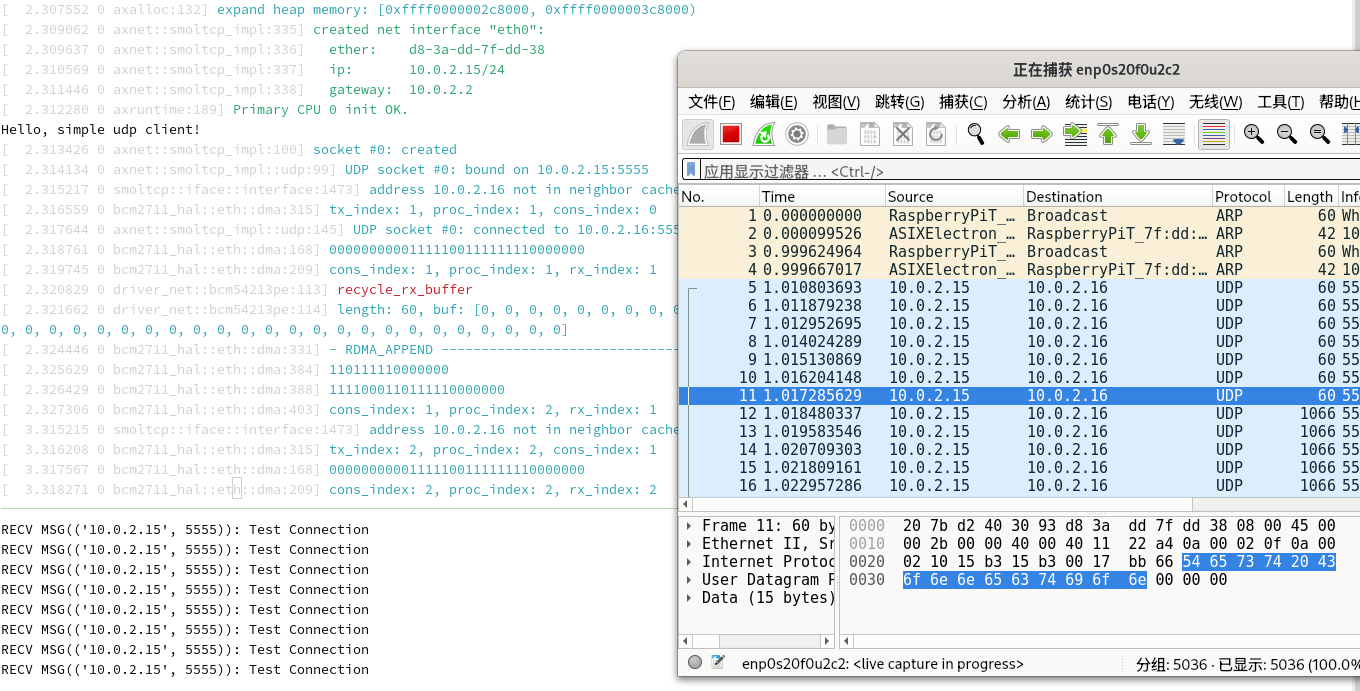
\includegraphics[width=\textwidth]{./imgs/测试-udp发包正常.png}
        \caption{Udp发包正常}    \label{test::Udp发包}
    \end{figure}   

    \subsubsection{Udp 收包测试}

    UdpSocket 收包测试我主要根据两种常见的网络联通方式进行测试,即 Netcat 和 ping。
    首先,针对 ARP,ICMP 包的测试(如图\ref{test::pingICMP回返测试}所示)。
    其中左上角是串口面板,右上角是正在运行中的 server.py 程序,左下角是
    执行的指令,即 ping 10.0.2.15。
    
    根据 ping 的一般操作流程,首先上位机中会先通过 ARP 探寻包,询问 10.0.2.15
    IP 地址所对应的硬件 MAC 地址,在下位机回返 MAC 地址后,连接被建立。
    上位机发送 ICMP Echo 请求到下位机,下位机以太网协议栈对收到的 ICMP 包进行处理,
    发送 ICMP Echo 作为回复。

    \begin{figure}[ht]
        \centering
        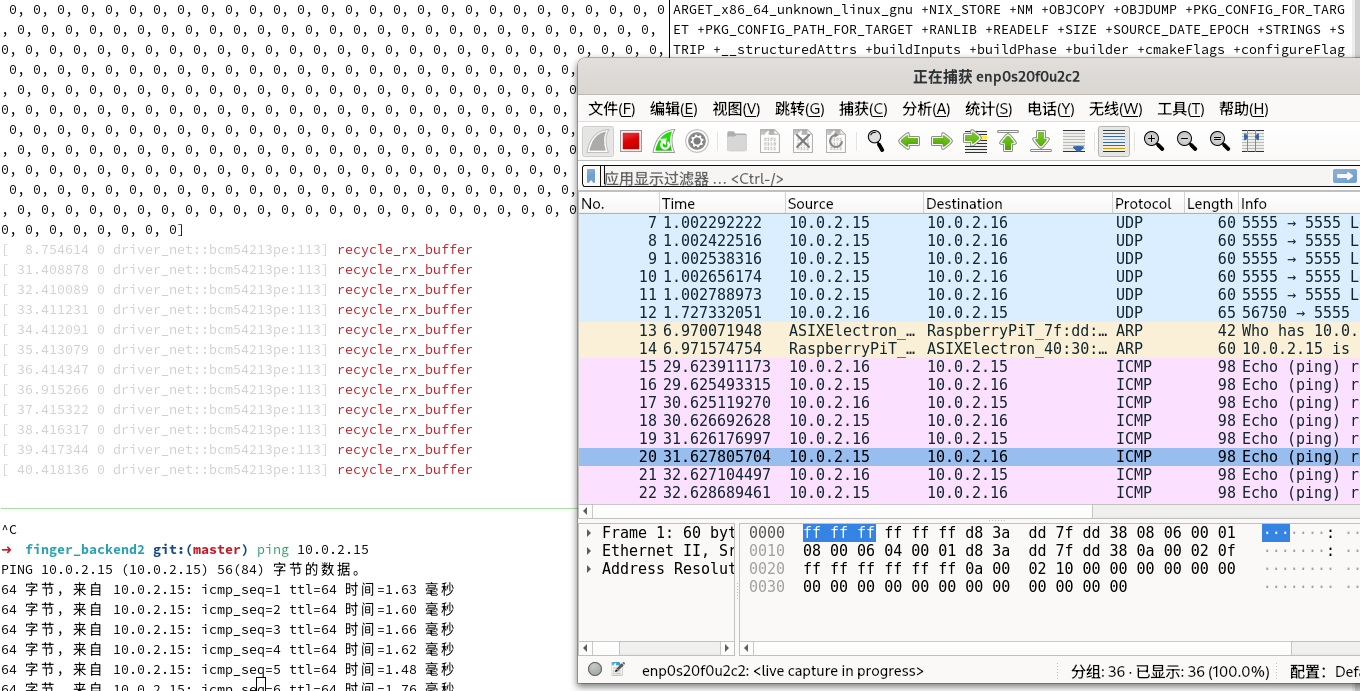
\includegraphics[width=\textwidth]{./imgs/测试-pingICMP回返测试.png}
        \caption{ping 回返测试}    \label{test::pingICMP回返测试}
    \end{figure}   

    然后,根据指纹考勤系统由上位机经由网络向下位机发送指纹信息的需求,
    我对于 Udp 连接进行了简单的测试。即通过 netcat 直接将一个字节数组
    (指纹模块的 LED 控制信号)
    由上位机传输到下位机,由图\ref{test::接收netcat数据}所示,下位机中
    缓冲区的字节数据与上位机中通过 netcat 传输的字节数据完全一致
    \footnote{这个地方没有对边界进行判断,直接打印了整个缓冲区}。

    \begin{figure}[H]
        \centering
        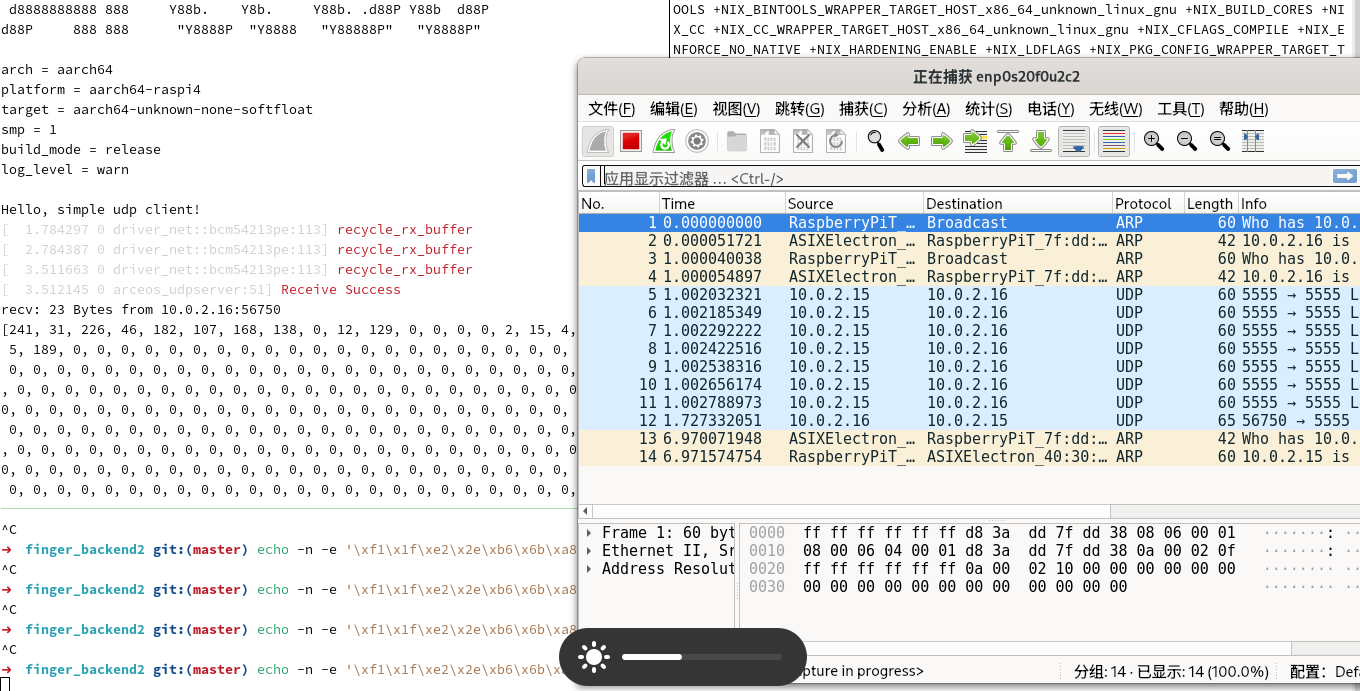
\includegraphics[width=\textwidth]{./imgs/测试-接收netcat数据.png}
        \caption{接收netcat数据}    \label{test::接收netcat数据}
    \end{figure}   

    \subsubsection{传输速率测试}
    
    在进行 UDP 层面传输速率测试的时候,在物理层面上采用类似前章节中对以太网帧进行测试时的连接结构。
    同时,软件层面上额外在上位机 10.0.2.16 中运行打开特定端口的程序避免出现报错返回包,直接通过 wireshark 对于收到的数据包
    数量进行记录(测试记录见附录表 2-3 \ref{tests::ArceOS-UDP传输速率测试})。
    
    其中采用的数据传输速率计算方法如下,其中 total\_bytes = UDP数据包数据部分长度 * 收发包数量,将收发包结果与前文中以太网帧
    层面的测试结果进行对比(如图 \ref{tests::ArceOSUDPETH对比图} 所示),可以明显发现 以太网帧传输速率 与 UDP帧传输速率存在较大差距,
    可以明显发现二者之间存在较大差距。

    根据初步的分析可能有两种原因导致这样的结果,由于 axnet, BCM54213PE 驱动兼容层的实现不正确损失了性能,或者是在 axnet 基于
    smoltcp 实现的网络协议栈中由于实现或者重复发包导致了性能损失。
    
    $$\text{mbps} = \frac{\text{total\_bytes} \times 8.0}{\text{elapsed\_secs} \times 1,000,000.0}$$

    \begin{figure}[H]
    \begin{tikzpicture}
        \centering
        \begin{axis}[
            xlabel={UDP 数据位长度}, ylabel={传输速率},
            xmin=0,
            width=0.8\textwidth,
            legend pos=north west,
            grid=both
        ]
        
        \addplot[name path=linux, thick, mark=*, orange] coordinates {
            (60, 189.773072)
            (128, 365.4372917)
            (256, 685.4498305)
            (384, 937.4238723)
            (512, 950.7467263)
            (768, 966.6822143)
            (1024, 973.7869313)
            (1280, 974.960128)
            (1408, 975.087309)
            (1500, 979.688400)
        };
        \addlegendentry{Linux 驱动}
        
        \addplot[name path=arceos, thick, mark=*, blue] coordinates {
            (128, 7.163255467)
            (256, 11.7116928)
            (384, 19.4936832)
            (512, 28.20819627)
            (640, 35.10186667)
            (768, 37.184256)
            (896, 46.4930816)
            (1024, 54.84489387)
            (1280, 65.50016)
            (1408, 72.410624)
            (1500, 0)
        };
        \addlegendentry{UDP 传输速率}

        \addplot fill between[
            of = linux and arceos,
            soft clip={domain=0:1500},
            every even segment/.style  = {gray,opacity=.4}
        ];

        \end{axis}
    \end{tikzpicture}
    \caption{ArceOS-UDP Eth对比图} \label{tests::ArceOSUDPETH对比图}
    \end{figure}
    
    \subsection{集成测试}

    集成测试部分主要测试了整个指纹考勤系统的集成功能,根据前文所提到的总体设计图,分为两个部分进行测试(如图 \ref{集成测试示意图} 所示)
    其中黄色部分被涵盖在指纹打卡及信息上传部分,红色部分被涵盖在指纹同步部分。

    \begin{figure}[ht]
        \centering
        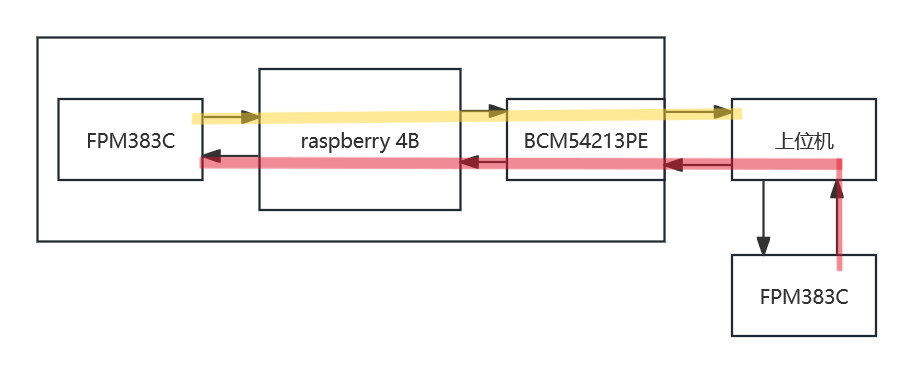
\includegraphics[scale=0.6]{./imgs/总体设计图-plus.png}
        \caption{集成测试示意图} \label{集成测试示意图}
    \end{figure}

    \subsubsection*{测试准备:}

    按照前文中测试脚本测试时使用的外部网线连接方式(如下图 \ref{集成测试连接图} 所示),将树莓派与测试主机连接到一起。
    在测试主机中运行 server.py 应用程序,该应用程序会打开对于当前主机 5555 端口的监听,并且自动分析在当前端口下的数据通信。


    根据设定,该端口会自动分析应用程序发来的 UDP 包究竟是用于测试连通性的 TEST\_CONNECTION 还是下位机汇报某指纹 ID 实现打卡成功的 PUNCH\_RECEIVED 包,
    根据其类型做出不同的处理,并且返回对应的信息。

    \begin{figure}[ht]
        \centering
        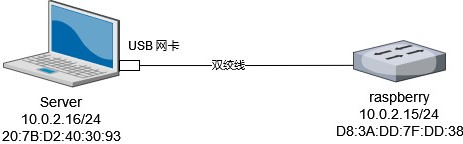
\includegraphics{./imgs/集成测试连接图.jpg}
        \caption{集成测试连接图} \label{集成测试连接图}
    \end{figure}

    \subsubsection{指纹打卡及信息上传}

    根据设计要求,在一般情况下,树莓派中不断轮询指纹识别模块,在指纹识别模块收到正确匹配信号之后,提取对应 UART帧 中保存的指纹 ID 数据,将此数据写入到 PUNCH\_RECEIVED 的
    ASCII 码中,直接通过 UDP 发送裸字节包到上位机中运行的 server.py 应用程序,在该应用程序中自动对 PUNCH\_RECEIVED 前缀进行识别,识别成功之后查询数据库,给该指纹 ID
    所对应的用户添加打卡记录。

    \begin{figure}[ht]
        \centering
        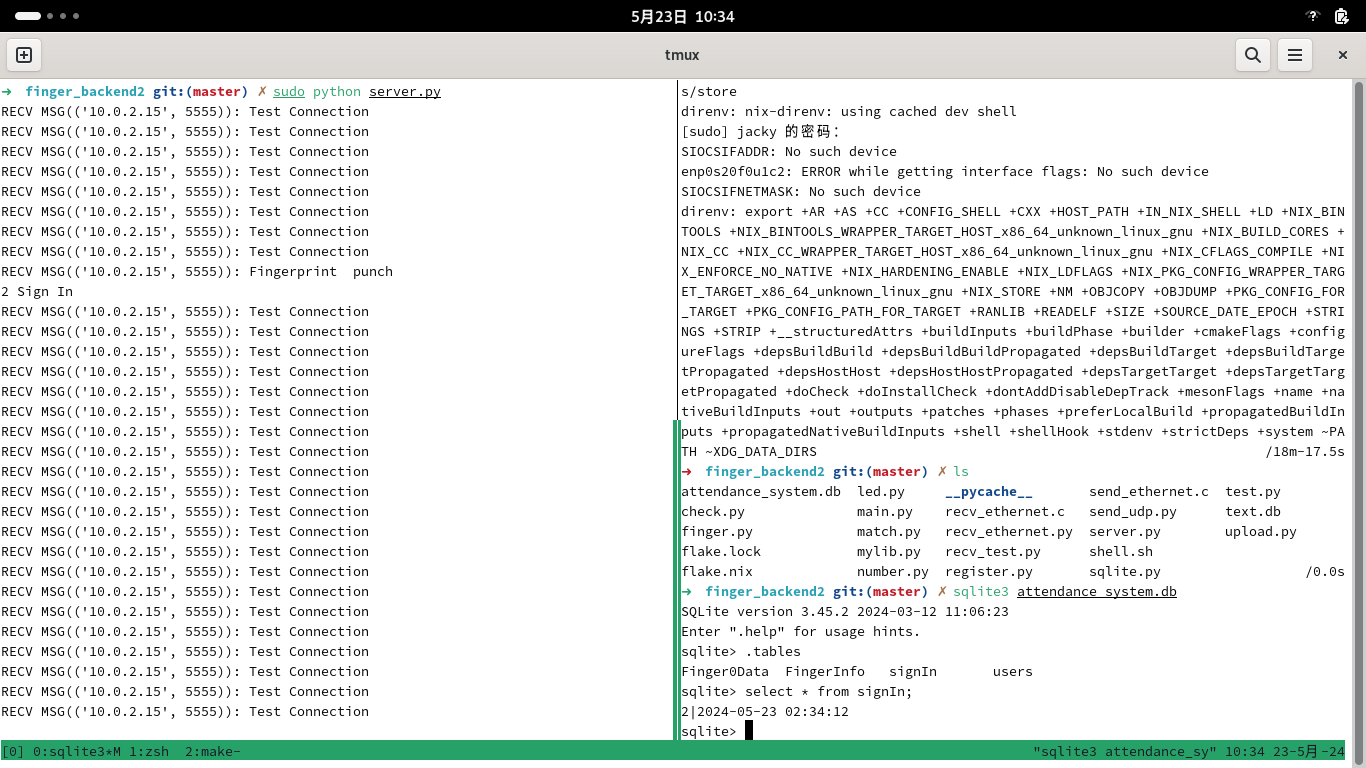
\includegraphics[width=\textwidth]{./imgs/集成测试-打卡信息上传.png}
        \caption{打卡信息上传示意图} \label{打卡信息上传示意图}
    \end{figure}

    如图 \ref{打卡信息上传示意图} 所示,左侧运行的 server.py 应用程序在对于当前网络下的 UDP 
    传输进行监听的时候,收到了两种不同的数据包 TEST\_CONNECTION 和 PUNCH\_RECEIVED
    当收到下位机打卡信息汇报之后,根据 FingerInfo 表查询指纹 ID 对应的用户名称,并将对应用户的打卡
    信息写入到 signIn 数据库。如图 \ref{打卡信息上传示意图} 右侧所示,
    在 signIn 数据库中以 CURRENT\_TIMESTAMP 的方式保存对应的打卡信息,
    打卡时间以上位机当前时间戳对应的格林尼治时间进行显示(在进行测试的时候上位机位于东八区)。

    \subsubsection{指纹同步}

    指纹同步测试在 \href{https://bitbucket.org/jackyliu16/arceos/commits/4554a70c7b902b3fcae488e9507377aff42fedd9}{arceos-4554a70} 提交中展开,
    其中使用的脚本在 \href{https://bitbucket.org/jackyliu16/attendance_system_backend/commits/921212f1f126da11868c32f7cba1502972fd6576}{backend-921212f}。
    在测试开始前清空树莓派从属指纹识别模块中的指纹模板(如图 \ref{tests::清空指纹模板})。
    在测试的时候,在上位机中打开 server.py 避免 5555 端口未被监听的报错,在树莓派商店,串口载入对应镜像完成之后,运行 mylib.py 中的同步测试命令,该命令会将
    当前数据库中保存的指纹特征数据下发到树莓派从属指纹识别模块中。

    \begin{figure}[ht]
        \centering
        \begin{subfigure}
            \centering
            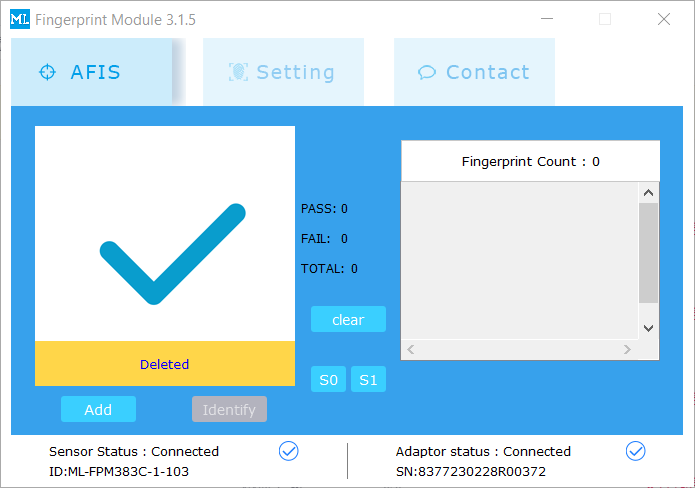
\includegraphics[width=\textwidth]{./imgs/清空指纹模板.png}
        \end{subfigure}
        \caption{清空指纹模板} \label{tests::清空指纹模板}
        \hfill
        \begin{subfigure}
            \centering
            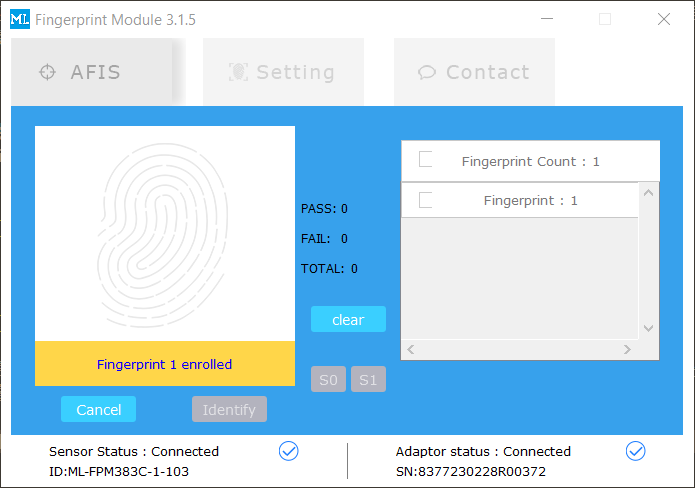
\includegraphics[width=\textwidth]{./imgs/注册指纹.png}
        \end{subfigure}
        \caption{指纹下载成功} \label{tests::指纹下载成功}
    \end{figure}

    根据当前胶水层(数据链路层与ArceOS 上层网络协议栈嵌合层)实现情况,目前尚没有办法能较好的处理将 UDP 存放到缓冲区中的问题,因此在指纹同步测试部分采用了一个相对较为简易的解决办法,
    即通过给两端添加延时来实现 UDP 收发包双端的同步。

    根据树莓派下位机中运行的嵌入式设备主循环 (见代码段 \ref{algorithm::fingerprint_network_comm}),在 local\_socket.recv\_from(\&mut buf) 从 ArceOS 上层网络协议栈中获取到第一个 UDP 包之后,
    应当进入一个持续的接受状态
    \footnote{根据 FPM383C 通信协议,下发指纹特征信息时,需要先发送指纹特征信息下载包,向指纹识别模块说明下载情况,然后上位机需要连续向下位机中发送多个固定长度(128)的指纹特征信息包},
    因此,在判定进入接收状态之后,主循环自动跳过指纹匹配\footnote{指纹下载过程不能被指纹匹配命令打断}后,继续接受并转发下一个 UDP 包,直到完成全部包的接受。

    在实际进行测试的时,发现现有串口传输驱动虽然可以实现简单的发送,解析与接受效果,但在面临连续发送较长字节时仍存在溢出问题。
    具体表现在传输常见 LED 控制信号(长度 22 字节),或者指纹特征信息下载包(长度 23 字节)时可以正常发送,但是在传输指纹特征数据下载包(长度 148 字节)时会出现由于部分字节没有正确传输,
    使指纹识别模块误认为传输还没有终止的死锁状态。
    
    交叉对比同一抽象类 SenderInterface 下的 SerialSender,UdpSocketSender 实现的效果及输出结果可以认为二者传输的数据是等价的,考虑到
    在实现串口传输驱动的时候采用的是 FIFO 方式实现的对应操作,在实际发送数据的时候可能因没能及时清空缓冲区导致溢出丢失字节进而导致死锁,手动在每次发送字节时添加了 50\_0000 纳秒的延迟后
    能正常传输较大字节数据。在包级别比对之后,发现在正常传输数据时,在树莓派端 recv\_from 处所接收到的包存在丢包情况。
    但是在启用 socket blocking 模式下无法复现该情况,初步认为该情况可能与尚未完整实现的胶水层有关(RxToken,TxToken中牵涉到 recycle 的问题),同时由于目前尚未实现多线程,在主循环上使用阻塞收报
    方式会导致死锁问题而无法避免使用 nonblocking socket。最终在 UDP 发包端每次发包间隔 0.092s,每次串口发送字节间隔 50\_0000 纳秒的情况下实现了最为基础的指纹同步功能。

    最终,在 mylib 测试脚本中携带的指纹模板总数探测包返回当前存在一个指纹模板,同时将 FPM383C 指纹模板切换到 PC 机中,对应的指纹模板也能够正常被检出(如图 \ref{tests::指纹下载成功})。
    


